\documentclass[tikz,border=10pt]{standalone}
\begin{document}
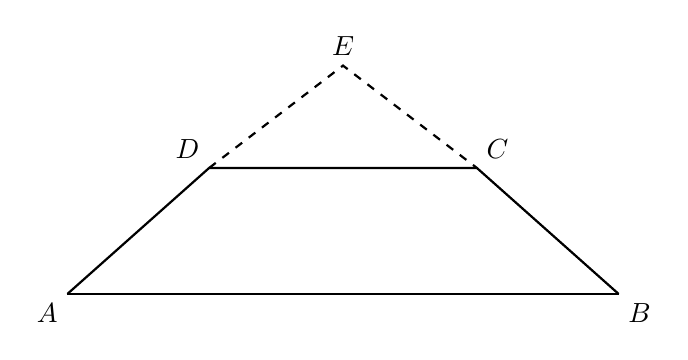
\begin{tikzpicture}
\coordinate (A) at (0,0);
\coordinate (B) at (7,0);
\coordinate (D) at (1.8,1.6);
\coordinate (C) at (5.2,1.6);
\coordinate (E) at (3.5,2.9);

\draw[thick] (A) -- (B);
\draw[thick] (A) -- (D) -- (C) -- (B);
\draw[thick,dashed] (D) -- (E) -- (C);

\node[below left] at (A) {$A$};
\node[below right] at (B) {$B$};
\node[above left] at (D) {$D$};
\node[above right] at (C) {$C$};
\node[above] at (E) {$E$};
\end{tikzpicture}
\end{document}
